% Cono de luz del espacio de Minkowski (x0=ct vs x)
\documentclass[border=4pt]{standalone}
\usepackage{tikz}
\usetikzlibrary{arrows.meta, calc}
\begin{document}
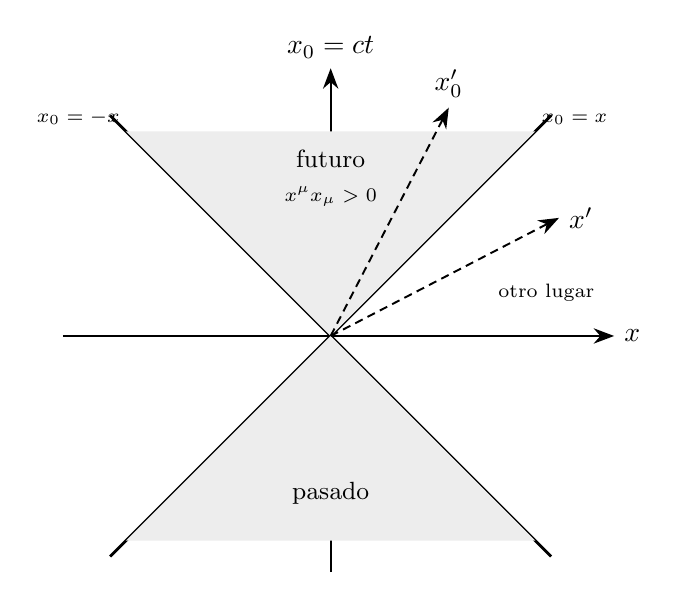
\begin{tikzpicture}[>={Stealth[length=2.6mm]}, line width=0.7pt]
  % ejes
  \draw[->] (-3.4,0)--(3.6,0) node[right]{$x$};
  \draw[->] (0,-3.0)--(0,3.4) node[above]{$x_0=ct$};
  % lineas de luz (x0 = +-x)
  \draw[line width=1pt] (-2.8,-2.8)--(2.8,2.8);
  \draw[line width=1pt] (-2.8,2.8)--(2.8,-2.8);
  % region futuro/pasado (sombreada suave)
  \fill[black!7] (0,0)--(2.6,2.6)--(-2.6,2.6)--cycle;
  \fill[black!7] (0,0)--(2.6,-2.6)--(-2.6,-2.6)--cycle;
  % etiquetas
  \node[align=center] at (0,2.0){\small futuro\\\scriptsize$x^\mu x_\mu>0$};
  \node[align=center] at (0,-2.0){\small pasado};
  \node[align=center, right] at (2.0,0.55){\scriptsize otro lugar};
  \node[above right] at (2.55,2.55){\scriptsize$x_0=x$};
  \node[above left] at (-2.55,2.55){\scriptsize$x_0=-x$};
  % ejes primados (boost): inclinados hacia el cono
  \draw[->, densely dashed] (0,0)--(2.9,1.5) node[right]{$x'$};
  \draw[->, densely dashed] (0,0)--(1.5,2.9) node[above]{$x'_0$};
\end{tikzpicture}
\end{document}
